\begin{surferPage}[Cayley-Cubic]{سطح كايلي التكعيبي \textenglish{(Cayley Cubic)}}
    هذا السطح التكعيبي (سطح درجته  $ 3 $) موجود أيضاً في جاليريا السطوح البسيطة.
      فهو يملك بالإجمال اربع متفردات من مخاريط مزدوجة.
   تمت تسيمته على إسم أرثور كايلي
   
    \textenglish{(Arthur Cayley)}
     الذي قام بالكثير من الأبحاث حول السطوح التكعيبية في القرن التاسع عشر.
    
    ولكن لودويج سكلافلي 
    \textenglish{(Ludwig Schläfli)} هو من قام لأول مرة في العام 1863 بتصنيف هذه السطوح بطريقة منهجية وبحسب عدد متفرداتها المحتملة. فعلى سبيل المثال، نقرأ في مقاله لماذا لا يمكن أن يكون لسطح تكعيبي أكثر من $4$ متفردات. هذا يعطي: $\mu(3)=4$. 
    
    حوالي العام 1900، درس فيلكس كلاين 
    \textenglish{(Felix Klein)}
     الأشكال المحتملة للسطوح التكعيبية الحقيقية؛ أراد ان يجيب على هذا السؤال إنطلاقاً من سطح كايلي التكعيبي بإعطائه تشويهات صغيرة:
    من خلال توسيع متفردات المخروط المزدوج، بفصل أو دمج
الأجزاء، تمكن في الواقع من العثور على جميع الأشكال الممكنة؛ هنا البعض منها:
    \vspace{0.3cm}
     \begin{center}
      \vspace{-0.2cm}
      \begin{tabular}{@{}c@{\ }c@{\ }c@{\ }c@{}}
        \begin{tabular}{@{}c@{}}
          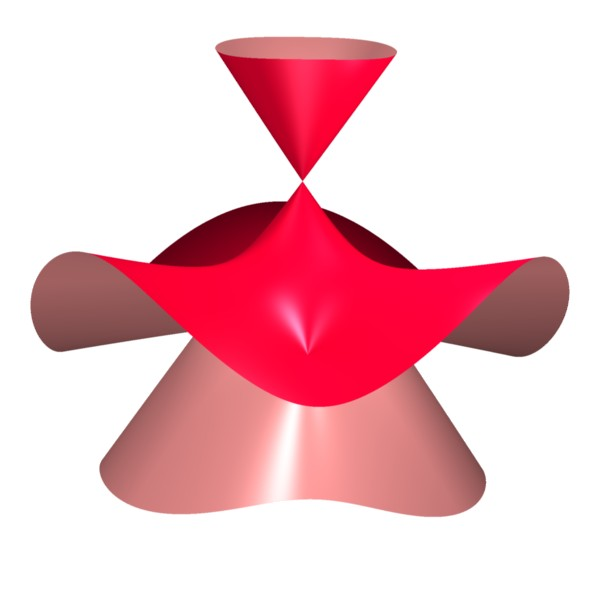
\includegraphics[width=1.35cm]{./../../common/images/cayley_cubic_0}
        \end{tabular}
        &
        \begin{tabular}{@{}c@{}}
          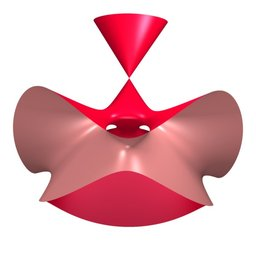
\includegraphics[width=1.35cm]{./../../common/images/cayley_cubic_1}
        \end{tabular}
        &
        \begin{tabular}{@{}c@{}}
          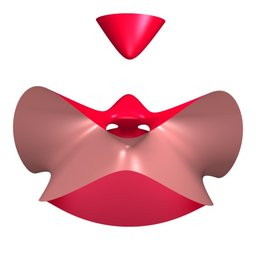
\includegraphics[width=1.35cm]{./../../common/images/cayley_cubic_2}
        \end{tabular}
        &
        \begin{tabular}{@{}c@{}}
          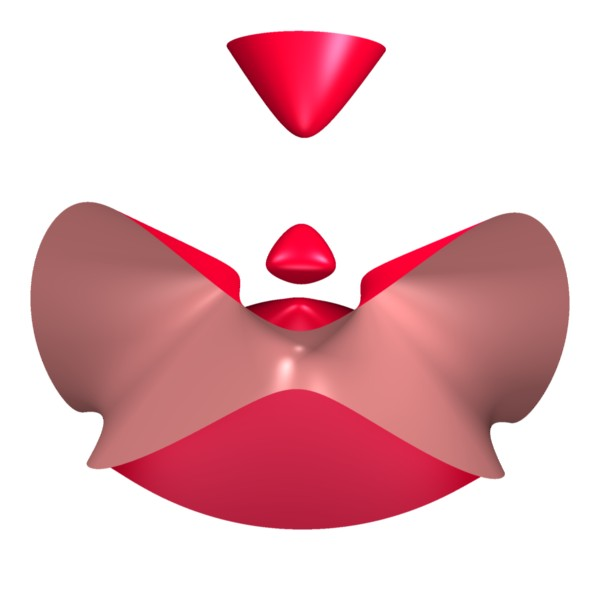
\includegraphics[width=1.35cm]{./../../common/images/cayley_cubic_3}
        \end{tabular}
      \end{tabular}
    \end{center}
\end{surferPage}
